%
% Bachelorarbeit
% Phil Diegmann
%

% -----------
% 1. Präambel
% -----------

% Allgemeine Einstellungen
% ------------------------
\documentclass[
    pdftex,
	a4paper,
	oneside,
	12pt,
	liststotocnumbered
]{article}
\usepackage{times}            % Times New Roman

\usepackage[utf8]{inputenc}   % utf-8
\usepackage[T1]{fontenc}      % Umlauttrennung
\usepackage[german]{babel}    % deutsche Silbentrennung
\selectlanguage{german}       % deutsche Betitelung
\usepackage{nicefrac}

% Titel-Font-Größen
\usepackage{titlesec}
\titleformat{\section}{\bfseries}{\thesection.}{12pt}{}
\titleformat{\subsection}{\bfseries}{\thesubsection }{12pt}{}

% Seitenränder
\usepackage[
    top=2.5cm, 
    bottom=2.5cm, 
    left=5cm, 
    right=1cm
]{geometry} 

% Fussnoten
\usepackage[hang,flushmargin]{footmisc}    
\renewcommand*{\footnotelayout}{\footnotesize} % size of text
\renewcommand{\footnotemargin}{2.2em}          % margin between text and number
\setlength{\footnotesep}{1.3em}                % space between footnotes
\setlength{\skip\footins}{2.5em}               % space between text & footnotes
\usepackage{savefnmark}

% Abkürzungen
\usepackage[printonlyused]{acronym}    
\renewcommand{\bflabel}[1]{{#1\hfill}}

% Seitennummerierung oben
\usepackage{scrpage2} 
\usepackage[dvips]{color}
\clearscrheadfoot 
\chead[\pagemark]{\textcolor[gray]{0.5}{\pagemark}} 
\pagestyle{scrheadings}

% TOC, LOF, FIG Styles
\usepackage{tocloft, titletoc}  
\setlength{\cftaftertoctitleskip}{0em}
\renewcommand{\cftloftitlefont}{\bfseries}
%\renewcommand{\cftfigfont}{\bfseries}
\renewcommand{\cfttoctitlefont}{\bfseries}
\renewcommand{\cftlottitlefont}{\bfseries}
\titlecontents{section}     % set formatting for \section 
[2.3em]                     % adjust left margin
{\vspace{0.5em}}            % font formatting
{\hspace{-1.8em}.\contentslabel{0.7em}\hspace{1em}} % section label and offset
{\hspace*{-2.3em}}
{\titlerule*[1mm]{.}\contentspage}

\titlecontents{subsection}  % set formatting for \subsection 
[3em]                       % adjust left margin
{\vspace{0.5em}}            % font formatting
{\contentslabel{2.3em}}     % section label and offset
{\hspace*{-2.3em}}
{\titlerule*[1mm]{.}\contentspage}

\titlecontents{subsubsection}  % set formatting for \subsubsection 
[4.2em]                       % adjust left margin
{\vspace{0.5em}}            % font formatting
{\contentslabel{2.3em}}     % section label and offset
{\hspace*{-2.3em}}
{\titlerule*[1mm]{.}\contentspage}

\titlecontents{figure}      % set formatting for \subsection 
[2.3em]                     % adjust left margin
{\vspace{0.5em}}            % font formatting
{\contentslabel{2.3em}}     % section label and offset
{\hspace*{-2.3em}}
{\titlerule*[1mm]{.}\contentspage}

\titlecontents{table}       % set formatting for \subsection 
[3.4em]                     % adjust left margin
{\vspace{0.5em}}            % font formatting
{:\hspace*{0.9em}\contentslabel{4.5em}}     % section label and offset
{\hspace*{-2.3em}}
{\titlerule*[1mm]{.}\contentspage}


% Literaturverzeichnis
\usepackage[
    bibstyle=authortitle,   %  in Verzeichnis das Jahr nicht hinter Autoren anzeigen
    citestyle=authoryear,   % in Fussnote das Jahr mit anzeigen
    isbn=false,             % keine ISBN-Nummer
    url=false,              % keine URLs
    doi=false,              % keine DOI
    maxcitenames=1,         % nur einen Autor in Fussnote anzeigen
    maxbibnames=30          % alle Autoren vor Titel anzeigen
]{biblatex}
\addbibresource{literature.bib}
\let\cite\textcite

\usepackage{caption}
\usepackage{chngcntr}

% Tabellenpackete
\usepackage{array}
\usepackage{xcolor}
\usepackage{longtable}
\usepackage{setspace}
\counterwithin{table}{section}
\usepackage{multirow}

% Grafiken anzeigen
\usepackage[pdftex]{graphicx}
\graphicspath{{figures}}
\counterwithin{figure}{section}
\usepackage[absolute,overlay]{textpos}

\begin{document}

\shorthandoff{"}

% Renews
\renewcommand{\figurename}{Abb.}
\renewcommand{\tablename}{}
\renewcommand\thefigure{\arabic{section}-\arabic{figure}}
\renewcommand\thetable{Tab. \arabic{section}-\arabic{table}}
\newcommand{\todo}[1]{\textbf{\textsc{\textcolor{red}{TODO: #1}}}}

% Variables
\newcommand{\CC}{Cloud Computing }
\newcommand{\CCs}{Cloud Computings }
\newcommand{\CCComma}{Cloud Computing, }
\newcommand{\TCC}{Themengebiet Cloud Computing }
\newcommand{\HiTCC}{Herausforderungen im Themengebiet Cloud Computing }
\newcommand{\TCCComma}{Themengebiet Cloud Computing, }
\newcommand{\CSP}{Cloud-Service-Provider }
\newcommand{\CSPComma}{Cloud-Service-Provider, }
\newcommand{\CSPDot}{Cloud-Service-Provider. }
\newcommand{\CSPn}{Cloud-Service-Providern }
\newcommand{\CSp}{Cloud-Service-Provider}
\newcommand{\CSPs}{Cloud-Service-Providers }
\newcommand{\CSPsDot}{Cloud-Service-Providers. }
\newcommand{\CSPsComma}{Cloud-Service-Providers, }
\newcommand{\CSU}{Cloud-Service-Nutzer }
\newcommand{\CSUDot}{Cloud-Service-Nutzer. }
\newcommand{\CSUs}{Cloud-Service-Nutzers }
\newcommand{\CSUn}{Cloud-Service-Nutzern }
\newcommand{\CSUComma}{Cloud-Service-Nutzer, }
\newcommand{\CSUsComma}{Cloud-Service-Nutzers, }
\newcommand{\CSUsDot}{Cloud-Service-Nutzers. }
\newcommand{\CSUnDot}{Cloud-Service-Nutzern. }
\newcommand{\CS}{Cloud-Service }
\newcommand{\Cs}{Cloud-Service}
\newcommand{\CSComma}{Cloud-Service, }
\newcommand{\CSs}{Cloud-Services }

\pagenumbering{Roman}

% ---------
% Deckblatt
% ---------
\vspace*{1mm}

% Name
\thispagestyle{empty}
Phil Diegmann

\vspace*{23mm}

% Bacheloararbeit
\begin{center}
\textbf{
    Bachelorarbeit
\linebreak
    im Fach Allgemeine Wirtschaftsinformatik}
\end{center}

\vspace*{20mm}

% Titel
\begin{center}
\LARGE 
    Development of mHealth Apps – Discovering the Dos and Don'ts in the Case of ePill
\end{center}

\vspace*{8mm}

% Themensteller
\begin{center}
    Themensteller: Jun.-Prof. Dr. Ali Sunyaev
\end{center}

\vspace*{12mm}

% Vorgelegt
\begin{center}
    Vorgelegt in der Bachelorprüfung
\linebreak
    im Studiengang Wirtschaftsinformatik
\linebreak
    der Wirtschafts- und Sozialwissenschaftlichen Fakultät
\linebreak
    der Universität zu Köln
\end{center}

\vspace*{30mm}

% Köln, September 2013
\begin{center}
Köln, September 2013
\end{center}





% ------------------
% Inhaltsverzeichnis
% ------------------
\tocloftpagestyle{scrheadings}
\tableofcontents
\newpage

% ---------------------
% Abkürzungsverzeichnis
% ---------------------
\section*{Index of Abbreviations}
\addcontentsline{toc}{section}{Index of Abbreviations}
\begin{longtable}{@{}p{.275\textwidth}@{}p{.725\textwidth}@{}}
    app & Application \\
    app user & intended audience for the app \\
    CDN & Content Delivery Network. Multiple servers which are globally distributed for serving static content with high availability and performance \\
    CSS & Cascading Style Sheets. A language used to style web pages \\
    DNS & Domain Name System. Used to translate domain names into IP-Addresses \\
    eHealth & "a paradigm involving the concepts of health, technology, and commerce, with commerce and technology as tools in the service of health"\footnote{\cite{MartinezPerez.2013}, p. 2}. eHealth belongs to the field of telehealth.\footnote{cf. \cite{MartinezPerez.2013}, p. 2} \\
    ePill & a patient-centered health IT service which offers information on pharmaceuticals and aggregation of data in context\footnote{cf. \cite{Dehling.2012b}, p. 2} \\
    framework & can contain source code, tools and libraries, which together provide specific or common but abstracted functionality \\
    frontend & visible user interface for the app user \\
    HECAT & Health Education Curriculum Analysis Tool\footnote{\url{http://www.cdc.gov/HealthyYouth/HECAT/}} \\
    HIT & abbreviation for Health Information Technology \\
    HTML & HyperText Markup Language, a markup language to design web pages \\
    IDE & Integrated Development Environment \\
    JSON & JavaScript Object Notation, represents data structures \\
    mHealth & "medical and public health practice supported by mobile devices, such as mobile phones, patient monitoring devices, personal digital assistants (PDAs), and other wireless devices"\footnote{\cite{WorldHealthOrganization.2011} cited by \cite{MartinezPerez.2013}, p. 2}, also known as m-Health \\
    mHealth apps & "aim at providing seamless, global access to tailored health IT services and have the potential to alleviate global health burdens"\footnote{\cite{Dehling.2013}, p. 1} \\
    MVC & Model-View-Controller. A software architecture pattern which separates logic and user interfaces. Models are representatives of data structures. Views contains the user interface definitions and controllers contains the application logic \todo{cite} \\
    NDK & Native Development Kit. Bundled software and tools which enables the developer to implement programs on native-code languages\footnote{cf. \url{http://developer.android.com/tools/sdk/ndk/index.html}} \\
    OS & Operating System \\
    SDK & Software Development Kit. Bundled software and tools for developing with or for a specified OS or framework \\
    telehealth & delivery of medical- or health-related information or services via telecommunication technologies \\
    usability & "extent to which a product can be used by specified users to achieve specified goals with effectiveness, efficiency and satisfaction in a specified context of use"\footnote{\cite{Yeh.2012}, p. 64 as quoted from ISO 9241-11 (1998)} \\
    use value & the utility of consuming a good or service \\
    user interface & for humans visible controls and layout of an application \\
    W3C & World Wide Web Consortium\footnote{\url{http://www.w3.org}} \\
\end{longtable}

% -------------------
% Tabellenverzeichnis
% -------------------
\listoftables
\addcontentsline{toc}{section}{Tabellenverzeichnis}
\newpage

\normalsize
\setstretch{1,5}
\pagenumbering{arabic}

% ------
% Inhalt
% ---------
\section{Einleitung}
\subsection{Problemstellung}
\subsection{Zielsetzung}
\subsection{Was ist mHealth?}
\newpage
\section{The ePill System}

\subsection{The System in general}
The ePill system (http://epill.uni-koeln.de) was developed by the University of Cologne to improve the readability and comprehensibility of instruction leaflets of medical drugs. Additionally ePill aims to provide further information on adverse reactions and interactions of different medical drugs. ePill emphasizes an easy readability and access to informations.
\\
There are three major functions covered by the system: Searching for pharmaceuticals, display information on pharmaceuticals and supplementing services.\footnote{cf. for this section \cite{Dehling.2012}, p. 2} The search enables the user to find corresponding pharmaceuticals depending on specified parameters in the underlying database. As an extend, the display functionality enables the user to read the leaflet information in an optimized fashion. Finally supplementing services are provided to refine the displayed information (e.g. select the level of detail of the displayed information), linking pharmaceuticals as well as other information and aggregate pharmaceutical information (e.g. interactions).
\\
An integration and personalization depending on the current user's health records was not implemented due to the arising privacy and trust challenges.\footnote{cf. \cite{Kaletsch.2011} cited by \cite{Dehling.2012}, p. 2}\footnote{cf. \cite{Kaletsch.2011}, pp. 5-6}

\subsection{The Web Application}
The web application of the ePill system introduces itself highly customizable to the user. Right 
\newpage
\section{Mobile App-Entwicklung}
\subsection{Normen der mobilen App-Entwicklung}
\subsection{Best-Practices}
\newpage
\section{Die Entwicklung des mobilen ePill-Clients}
\subsection{Analyse}
\subsection{Planung}
\subsection{Design}
\subsection{Entwicklung}
\subsection{Tests}
\newpage
\section{Fazit}
\newpage

% --------------------
% Literaturverzeichnis
% --------------------
\newpage
\patchcmd{\bibsetup}{\interlinepenalty=5000}{\interlinepenalty=10000}{}{}
\printbibliography[title={Literaturverzeichnis}]
\addcontentsline{toc}{section}{Literaturverzeichnis}
\newpage

% ---------
% Anhang
% ---------
\section*{Erklärung}
\addcontentsline{toc}{section}{Erklärung}

Hiermit versichere ich an Eides Statt, dass ich die vorliegende Arbeit selbstständig und ohne die Benutzung anderer als der angegebenen Hilfsmittel angefertigt habe. 
Alle Stellen, die wörtlich oder sinngemäß aus veröffentlichten und nicht veröffentlichten Schriften entnommen wurden, sind als solche kenntlich gemacht. 
Die Arbeit ist in gleicher oder ähnlicher Form oder auszugsweise im Rahmen einer anderen Prüfung noch nicht vorgelegt worden.

\vspace{30mm}
\begin{flushleft}
    Köln, den 26. September 2013
\end{flushleft}
\section*{\hspace{0.2cm}Lebenslauf} 
\addcontentsline{toc}{section}{Lebenslauf}

\begin{flushleft}

% Persönliche Angaben
\begin{tabular}{p{11em} p{10em} p{10em}}
    \multirow{5}{*}{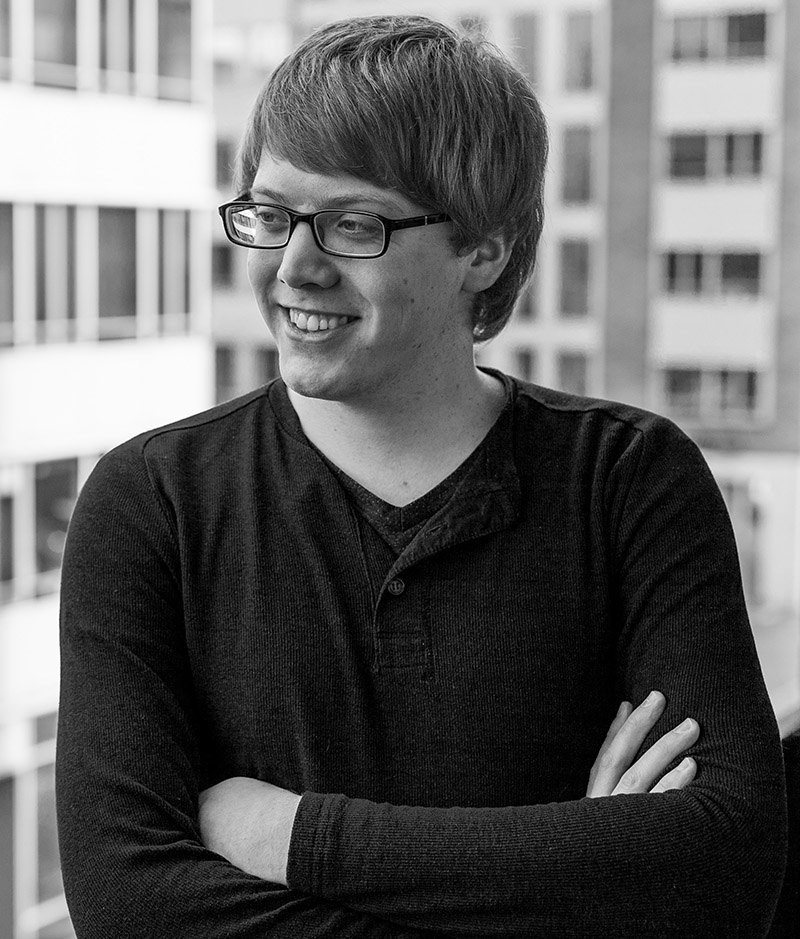
\includegraphics[width=40mm]{figures/passfoto.jpg}} & \textbf{Persönliche Angaben} & \addspace \\
    & Name: & Phil Diegmann \\
    & Anschrift: & Wipperfürther Str. 477, 51515 Kürten \\
    & Geburtsdatum und -ort: & 06.02.1991 in Wipperfürth \\
    & Familienstand: & ledig \\
\end{tabular}

\vspace{1.5em}

% Ausbildung
\begin{tabular}{p{11em} p{22.5em}}
    \textbf{Schulische Ausbildung} & \addspace \\
    1998 - 2002 & St. Antonius Grundschule in Wipperfürth \\
    2002 - 2010 & Engelbert-von-Berg Gymnasium in Wipperfürth, Abschluss: Abitur (1,5) \\
\end{tabular}

\vspace{0.5em}

% Studium
\begin{tabular}{p{11em} p{22.5em}}
    \textbf{Studium} & \addspace \\
    10/2010 - 09/2013 & Universität zu Köln, Wirtschaftsinformatik, Bachelor of Science \\
    10/2013 - 09/2015 & Universität zu Köln, Information Systems, Master of Science
\end{tabular}


\vspace{-1em}

% Praktika

% Beruflicher Werdegang

\end{flushleft}

\end{document}